\documentclass[22pt]{beamer}
\usepackage{textcomp}
\usepackage[orientation=portrait, size=custom, width=91.44, height=91.44,scale=1.3]{beamerposter} % 36in*2.5 = 90cm
\usepackage[absolute,overlay]{textpos}
\usepackage{bookmark} %pdflatex says to use this to avoid errors...
\usepackage{graphicx} %for including images
\graphicspath{{figs/}} %location of images
\usepackage{wrapfig} %wrap text around the images
\usepackage{listingsutf8}    
\usepackage{amsmath}
\usepackage{gensymb}
\usepackage[export]{adjustbox}
\usepackage[skins,theorems]{tcolorbox}
\usepackage{tikz}
\newcommand*\circled[1]{\tikz[baseline=(char.base)]{
            \node[shape=circle,draw,inner sep=2pt] (char) {#1};}}
\usepackage{array}
\usepackage{booktabs,adjustbox}
\usepackage{subcaption} 
\usepackage{amsmath,amsfonts}
\usepackage{MnSymbol}


\usetheme{Berlin}
\definecolor{MacBlue}{rgb}{0.10196,0.22353,0.53725}
\definecolor{MacMaroon} {rgb}{0.47843, 0, 0.23137}
\definecolor{MacMaroon2} {rgb}{0.47451, 0, 0}
\definecolor{MacGray}{rgb}{0.50196,0.49804,0.51765}
\definecolor{MacMaroon3}{rgb}{00.47,0.2,0.31}
\definecolor{MacGold}{rgb}{1, 0.75,0.35}
\usecolortheme[named=MacBlue]{structure}
\setbeamertemplate{caption}[numbered]
\setbeamertemplate{navigation symbols}{}

% -----------------------------------------------------------------------------------------------------------------
% For code snippet
\usepackage[utf8]{inputenc}

% Default fixed font does not support bold face
\DeclareFixedFont{\ttb}{T1}{txtt}{bx}{n}{12} % for bold
\DeclareFixedFont{\ttm}{T1}{txtt}{m}{n}{12}  % for normal

% Custom colors
\usepackage{color}
\definecolor{deepblue}{rgb}{0,0,0.5}
\definecolor{deepred}{rgb}{0.6,0,0}
\definecolor{deepgreen}{rgb}{0,0.5,0}
\usepackage{listings}

% Python style for highlighting
\newcommand\pythonstyle{\lstset{
%language=Python,
%basicstyle=\ttm,
%otherkeywords={self},             % Add keywords here
%keywordstyle=\ttb\color{deepblue},
%emph={MyClass,__init__, for},          % Custom highlighting
%emphstyle=\ttb\color{deepred},    % Custom highlighting style
%stringstyle=\color{deepgreen},
%frame=tb,                         % Any extra options here
%showstringspaces=false            % 
    language        = Python,
    basicstyle      = \ttfamily,
    keywordstyle    = \color{orange},
    keywordstyle    = [2] \color{teal}, % just to check that it works
    stringstyle     = \color{red},
    commentstyle    = \color{blue}\ttfamily
}}



% Python environment
\lstnewenvironment{python}[1][]
{
\pythonstyle
\lstset{#1}
}
{}

% Python for external files
\newcommand\pythonexternal[2][]{{
\pythonstyle
\lstinputlisting[#1]{#2}}}

% Python for inline
\newcommand\pythoninline[1]{{\pythonstyle\lstinline!#1!}}

% -----------------------------------------------------------------------------------------------------------------

%TODO:
%- bullet points
%
%Background
%- explain how algos work (this is the challenge)
%- discuss differences and argue why you chose which
%
%Testing
%- justify strings you chose
%
%Diagrams:
%-units
%
%Conclusion
%-in line with what other people reported?
%
%Future work:
%-either be specific or leave out



\title{Approximate Regular Expressions: A Comparison of Exact and Approximate Matching Algorithms}
\subtitle{}  
  \author[Gadriwala, Noshin \& Siddiqui]{Umme Salma Gadriwala, Tasnim Noshin, Rumsha Siddiqui \vspace{0.3cm} \newline \small \{gadriway, noshint, siddiqur\}@mcmaster.ca}
  \institute[McMaster University]{Department of Computing and Software, McMaster University

1280 Main St. W, Hamilton, Ontario, Canada L8S 4L8}
  \date{April 2019}

\begin{document}
\begin{frame}[fragile]

\begin{textblock}{2}(0.7,1)

\includegraphics[height=8.5cm]{englogo.png}
\end{textblock}

\begin{textblock}{8}(4,1)
\titlepage
\end{textblock}

\begin{textblock}{2}(12.7,0.75)

\includegraphics[height=12cm]{cslogo.png}
%\centering
%\textbf{Tweet us} \\
%your thoughts: \\
%{[worth pursuing?] [achievable?]}
%{\color{MacBlue} @TeamDeepCheck \#MacCSCapstone \#MacEng}
\end{textblock}

\begin{textblock}{7.25}(0.5,3.1)

\begin{block}{Motivation}
Applications of finding exact and approximate string matches range far and wide. In browsing, the find function is often employed to locate exact text snippets on a screen. In computer security, approximate matching is necessary to find computer viruses and spam signatures that resemble certain patterns. In bioinformatics, approximate matching is vital for comparing and contrasting DNA and protein sequences \cite{Approx1}. The length of sequences involved in these applications reach billions. Thus, efficient string matching algorithms are needed to preserve time and cost of resources.
\end{block}

\begin{block}{Problem}
 Different applications have different constraints on how strict of a match must be found. Some applications require both exact and approximate matching features. This project explores whether or not an implementation of exact matching can be replaced with one of approximate matching, where the error value for an exact match request would be set to zero. We aim to determine how an approximate matching algorithm fares in efficiency when compared to an exact matching algorithm.  
 %For ex: browser
 	% exact matching: ctrl-f to find text snippet
 	% approx. matching: allow for typos

\end{block}

\begin{block}{Solution}
A Python implementation of Thompson's exact matching algorithm is compared with that of Myers and Miller's approximate matching algorithm. Matches between string and regular expressions of various legnths are used for testing. The testing methodology compares the time each algorithm takes for the same samples. 
\end{block}


\begin{block}{Background Study}
\textbf{Exact Matching: Thompson's Algorithm}: This exact matcing algorithm generates a non-deterministic finite automata (NFA) from a given regular expression. The construction is O(m). The number states and transitions is O(m) as well, where m is the number of symbols \cite{Approx1}.

%\begin{figure}
%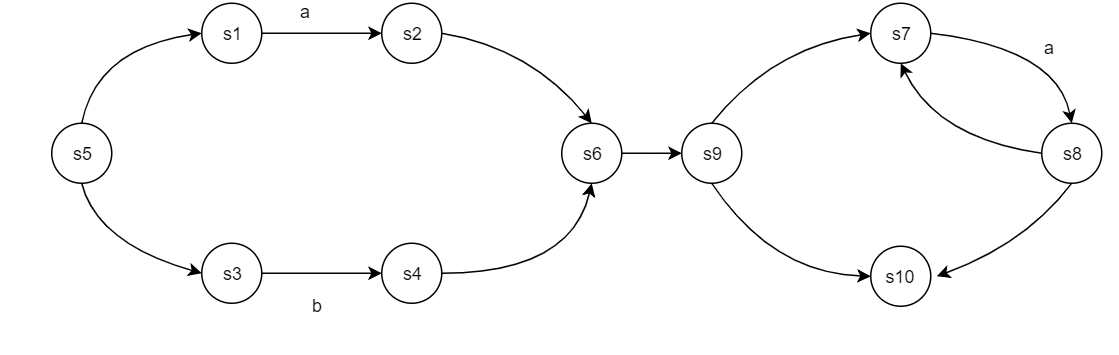
\includegraphics[scale=1.5]{ThompsonsNFA.PNG}
%\end{figure}

\vspace{5mm} %5mm vertical space

\textbf{Approximate Matching: Myers and Miller's Algorithm}: An approximate matching algorithms aims to find a match between a regular expression and a string with up to k errors. These k errors can consist of an insertion or deletion (a gap in the alignment of the regular expression and string), or a substitution (a difference in characters at a particular alignment position). The NFAs constructed in this approximate matching method are unique for each string and regular expression combination. The time complexity of Myers and Miller's is O(mn/k + m$2^{k}$ + (n + m) log m), where m and n are the lengths of the regular expession and string respectively. The space complexity is O($2^{k}$m), where k $<$= w, the word size \cite{Approx1}.


\begin{figure}
\raisebox{0.7\height}{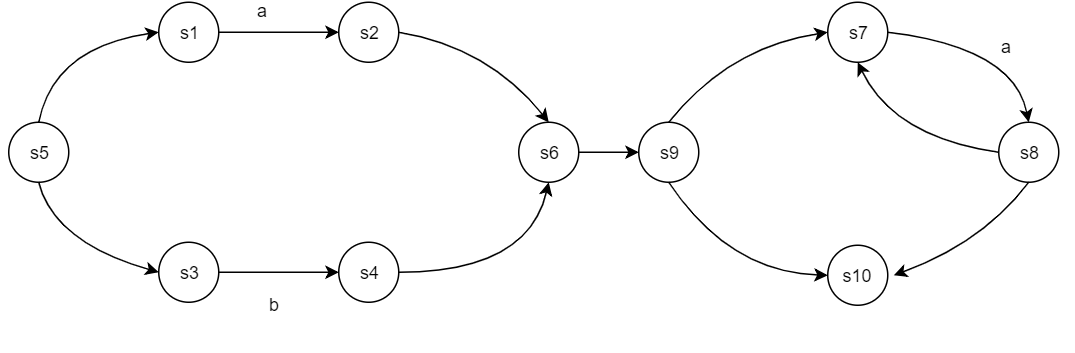
\includegraphics[scale=1.2]{ThompsonsNFAcropped.PNG}}
\hspace*{.2in}
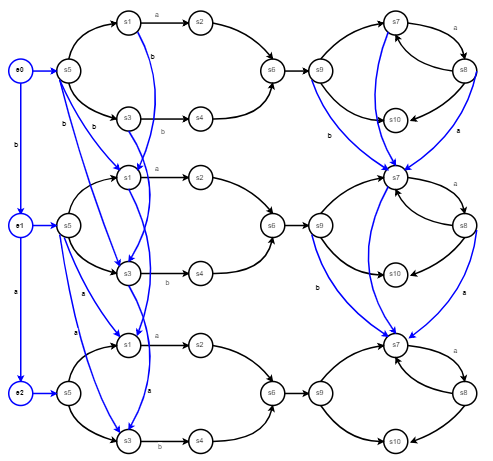
\includegraphics[scale=2]{MillerAndMyersAlgorithm.PNG}
\caption{The NFA on the left is constructed by Thompson's algorithm based on regular expression (a or b) a*. The NFA on the right is generated by Myers and Miller's algorithm based on the same regular expression, but specifically with string `ba'}
\end{figure}

\end{block}
\end{textblock}


\begin{textblock}{7.25}(8.25,3.1)
\begin{block}{Methodology}

\begin{python}
  # Sample: compute runtime of exact matching algorithm
  for i in range(numLength):
      # Extend the string
      string = string + "ab"*4
      start = time.time()
      for i in range(numIterations):
          exact_nfa.match(string)    
      end = time.time()
      # Compute average time to output
      exactTimes = exactTimes + [(end-start)/numIterations]
\end{python}


\begin{figure}
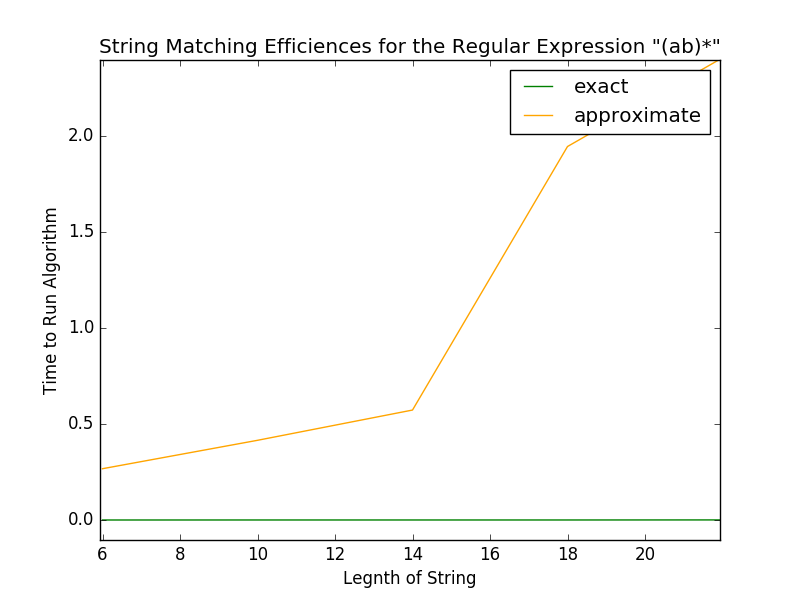
\includegraphics[scale=1.9]{result_2.PNG}
\caption{The time required to match strings of repeating sequences of `ab' to the regular expression `(ab)*', as the legnth of the string increases.}
\end{figure}


\end{block}


\begin{block}{Conclusions \& Future Work}
Based on the times computed through the experiment, it is evident that the approximate matching algorithm takes a significant amount of time. It is not worth the cost to use approximate matching for the case where k = 0. It is recommended to implement an exact matching algorithm to perform tasks that require exact matching. 

In this experiment, only two algorithms were explored. Future research would benefit from exploring the efficiency of a plethora of different methods.
\end{block}


\begin{block}{Acknowledgements}
We thank Dr. Sekerinski for inspiring this project, as well as his continued guidance in our learning and endeavours. We also thank Spencer Park and Erin Varey for their invaluable feedback and support. 
\end{block}

%--------------------------------------------
%REFERENCES
\begin{block}{References}
\setbeamertemplate{bibliography item}{\insertbiblabel}
\bibliographystyle{ieeetr}
{\scriptsize
\bibliography{bib}}
\end{block}

\begin{comment}
\begin{block}{References}
\setbeamertemplate{bibliography item}{\insertbiblabel}
\bibliographystyle{ieeetr}
{\scriptsize
\bibliography{bib}}
\end{block}
\vspace{-1.8mm}
\end{comment}
\end{textblock}

%
%\begin{textblock}{7.5}(0.5,14.6)
%\centering
%\textbf{Tweet us} \\
%your thoughts on DeepCheck and where you think the future of neural networks is headed \\
%{\color{MacBlue} @TeamDeepCheck \#MacCSCapstone \#MacEng}
%
%\end{textblock}

\end{frame}
\end{document}
